% !TeX TXS-program:compile = txs:///pdflatex/[--shell-escape]

\documentclass[11pt, letterpaper]{article}

\usepackage{minted}
\usepackage[utf8]{inputenc}
\usepackage[T1]{fontenc}
\usepackage{lmodern}
\usepackage{graphicx}
\usepackage{longtable}
\usepackage{wrapfig}
\usepackage{rotating}
\usepackage{amsmath}
\usepackage{textcomp}
\usepackage{amssymb}
\usepackage{hyperref}
\usepackage[round]{natbib}
\usepackage{subcaption}


\title{\bfseries Tarea}
\author{Ángel García Báez}
\date{\today}
\setcounter{tocdepth}{3} 

\begin{document}
	
	% Página de presentación
	\begin{titlepage}
		\centering
		\includegraphics[width=0.2\textwidth]{logo.png}\par
		\vspace{1cm}
		{\LARGE \bfseries Universidad Veracruzana \par}
		\vspace{1cm}
		{\Large Maestría en Inteligencia Artificial\par}
		\vspace{3cm}
		{\LARGE \bfseries Visión por Computadora \par}
		\vspace{1cm}
		{\Large \bfseries Examen de visión por computadora 1. Respuestas de los ejercicios practicos en MATLAB. \par}
		\vfill
		{\Large \textit{Ángel García Báez}\par}
		\vspace{1cm}
		{\Large Profesor: Dr. Héctor Acosta Mesa\par}
		\vfill
		{\Large \today \par}
	\end{titlepage}
	
	% Página exclusiva para la tabla de contenidos
	\newpage
	\tableofcontents
	\newpage
	
% Sección para el problema 1
\section{Objetivo de la práctica}

1.- Se tiene la siguiente imagen y se pide proponer y aplicar una técnica de transformación:

\begin{figure}[h!]
	\centering
	\begin{minipage}{0.8\textwidth}
		\centering
		\includegraphics[width=\textwidth]{Imagen1.png}
		\caption{Imagen 1.}
		\label{fig:Imagen 1}
	\end{minipage}\hfill
\end{figure}


2.- Se tienen las siguientes imágenes por lo que se desea aplicar un proceso de registro:

\begin{figure}[h!]
	\centering
	\begin{minipage}{0.48\textwidth} % Ajusta el ancho según necesites (menos de 0.5 para dejar espacio)
		\centering
		\includegraphics[width=\textwidth]{Imagen2_A.jpg}
		\caption{Imagen 2A.}
		\label{fig:imagen1}
	\end{minipage}\hfill % \hfill añade espacio horizontal entre los minipages
	\begin{minipage}{0.48\textwidth} % Ajusta el ancho según necesites
		\centering
		\includegraphics[width=\textwidth]{Imagen2_B.jpg}
		\caption{Imagen 2B.}
		\label{fig:imagen2}
	\end{minipage}
\end{figure}

\newpage

3.- Se tiene la siguiente imagen y se pide proponer una técnica de mejoramiento de la imagen:


\begin{figure}[h!]
	\centering
	\begin{minipage}{0.8\textwidth}
		\centering
		\includegraphics[width=\textwidth]{Imagen3.jpg}
		\caption{Imagen 3.}
		\label{fig:f3}
	\end{minipage}\hfill
\end{figure}



\newpage	
	
\section{Metodología y resultados}

\subsection{Procesos para la imagen 1}

Para aplicar una transformación sobre la imagen 1, primero se penso que necesita dicha imagen, es evidente que el contraste entre las montañas y el bosque es muy pronunciado, tanto que el bosque se ve mayormente negro al punto que no se pueden distinguir formas ni nada e incluso, se camuflajea un poco con el pueblo que se ve al fondo. Para poder solventar este contraste tan marcado entre los tonos de gris, se propone el uso de la ecualización por histograma para ampliar el rango de colores y poder distinguir mejor los elementos que estan presentes en la imagen.

Para ello se utilizo MATLAB haciendo uso del siguiente codigo:

\begin{minted}[linenos,firstnumber=1]{matlab}
%% Cargar imagen 1  
ruta1 = "imagen1.png";
I1 = imread(ruta1);
%% Aplicar el histograma %%
R1 = histeq(I1); 
%% Comparativa %%
subplot(1,2,1)
imshow(I1)
subplot(1,2,2)
imshow(R1)
\end{minted}

El resultado se muestra de la aplicación del histograma sobre la imagen se muestra en la siguiente comparativa

\begin{figure}[h!]
	\centering
	\begin{minipage}{0.48\textwidth} % Ajusta el ancho según necesites (menos de 0.5 para dejar espacio)
		\centering
		\includegraphics[width=\textwidth]{Imagen1.png}
		\caption{Imagen 1 base.}
		\label{fig:im1}
	\end{minipage}\hfill % \hfill añade espacio horizontal entre los minipages
	\begin{minipage}{0.48\textwidth} % Ajusta el ancho según necesites
		\centering
		\includegraphics[width=\textwidth]{R1.png}
		\caption{Ecualizada.}
		\label{fig:im1.1}
	\end{minipage}
\end{figure}


Logra distinguirse mejor los elementos que conforman al bosque pero se vuelven más borrosos los elementos del fondo.

\newpage	

\subsection{Procesos para la imagen 2}

Para la imagen 2, es necesario aplicar una transformación basada en la rotación de la imagen 2B para que quede igual que la imagen 1, para ello es necesario realizar un registro de landmarks que puedan guiar esta transformación afín, para facilitar las cosas se utilizarón las funciones que vienen en matlab adaptando codigo de clase:


\begin{minted}[linenos,firstnumber=1]{matlab}
%% Imagen 2 ESCANEO %%
original = imread("Imagen2_A.jpg"); % Reemplaza con la ruta de tu imagen de referencia
distorted = rgb2gray(imread("Imagen2_B.jpg")) ; % Reemplaza con la ruta de la imagen a registrar
%% Detect and extract features from both images.
ptsOriginal  = detectSURFFeatures(original);
ptsDistorted = detectSURFFeatures(distorted);
[featuresOriginal,validPtsOriginal] = ...
extractFeatures(original,ptsOriginal);
[featuresDistorted,validPtsDistorted] = ...
extractFeatures(distorted,ptsDistorted);
index_pairs = matchFeatures(featuresOriginal,featuresDistorted);
matchedPtsOriginal  = validPtsOriginal(index_pairs(:,1));
matchedPtsDistorted = validPtsDistorted(index_pairs(:,2));
%% Hacer el match %% 
showMatchedFeatures(original,distorted,...
matchedPtsOriginal,matchedPtsDistorted);
title('Matched SURF points,including outliers');
%% Excluir los outliers %%
[tform,inlierPtsDistorted,inlierPtsOriginal] = ...
estimateGeometricTransform(matchedPtsDistorted,matchedPtsOriginal,...
'similarity');
showMatchedFeatures(original,distorted,...
inlierPtsOriginal,inlierPtsDistorted);
title('Matched inlier points');
%% Recover the original image from the distorted image.
outputView = imref2d(size(original));
Ir = imwarp(distorted,tform,'OutputView',outputView);
imshow(Ir); 
title('Recovered image');
imshowpair(original,Ir)
\end{minted}

\newpage

Los resultados de aplicar el rastreo de los puntos y la transformación afín son los siguientes:

\begin{figure}[h!]
	\centering
	\begin{minipage}{0.48\textwidth} % Ajusta el ancho según necesites (menos de 0.5 para dejar espacio)
		\centering
		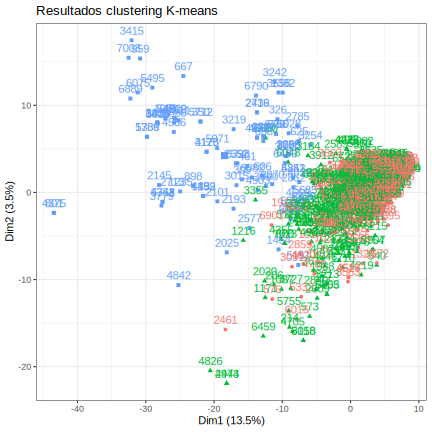
\includegraphics[width=\textwidth]{R2.png}
		\caption{Imagen con outliers.}
		\label{fig:im2}
	\end{minipage}\hfill % \hfill añade espacio horizontal entre los minipages
	\begin{minipage}{0.48\textwidth} % Ajusta el ancho según necesites
		\centering
		\includegraphics[width=\textwidth]{R3.png}
		\caption{Imagen sin outliers.}
		\label{fig:im2.2}
	\end{minipage}
\end{figure}



\begin{figure}[h!]
	\centering
	\begin{minipage}{0.7\textwidth}
		\centering
		\includegraphics[width=\textwidth]{R4.png}
		\caption{Superposición de la imagen original y la imagen transformada}
		\label{fig:f5}
	\end{minipage}\hfill
\end{figure}

Se observa como el algoritmo detecta automaticamente los puntos y sus coincidencias entre las imagenes y finalmente, la superposición de ambas, despues de rotar la segunda da como resultado la primera perfectamente.


\newpage
	
\subsection{Procesos para la imagen 3}

Para la imagen 3 que presenta un patron de circulos es necesario transformar la imagen y llevarla al dominio de las frecuencias con la transformada de fourier, donde se va a plicar un filtro pasa bajas para detectar esas frecuencias extrañas, para ello se determino un filtro gaussiano que detecta el centro en un a frecuencia de 50. Posteriormente se volvio la imagen del dominio de las frecuencias al dominio del espacio  , los resultados se muestran a continuación.

\begin{minted}[linenos,firstnumber=1]{matlab}
%% Cargar imagen 3 %%
ruta3 = "imagen3.jpg";
I3 = imread(ruta3);
gray = rgb2gray(I3);
imshow(I31)
%% Verlo con Fourier %%
% Transformada de Fourier centrada
F = fftshift(fft2(gray)); 
% fft2: calcula la transformada rápida de Fourier en 2D
% fftshift: mueve las bajas frecuencias al centro del espectro
% Obtener dimensiones de la imagen
[M, N] = size(gray);
% Crear una malla de coordenadas centradas
[u, v] = meshgrid(-N/2:N/2-1, -M/2:M/2-1); 
% u y v son coordenadas espaciales en el dominio de frecuencia
% centradas en (0,0) (el centro de la imagen)
% Calcular la distancia radial desde el centro para cada punto
D = sqrt(u.^2 + v.^2);
% Parámetro del filtro: radio de corte
D0 = 50; 
% Crear el filtro gaussiano pasa bajas
H = exp(-(D.^2) / (2 * D0^2)); 
% Este filtro deja pasar las frecuencias cercanas al centro (bajas)
% y atenúa las lejanas (altas)
% Aplicar el filtro en el dominio de la frecuencia
F_filtered = F .* H;
% Transformada inversa para volver al dominio espacial
img_filtered = real(ifft2(ifftshift(F_filtered))); 
% ifftshift: devuelve el centro al lugar original
% ifft2: transformada inversa de Fourier
% real: tomamos solo la parte real (por errores numéricos puede haber parte imaginaria)
% Normalizar la imagen resultante al rango 0-255
F2 = uint8(mat2gray(img_filtered) * 255); 
imshow(F2)
\end{minted}

\begin{figure}[h!]
\centering
\begin{minipage}{0.7\textwidth}
	\centering
	\includegraphics[width=\textwidth]{R5.png}
	\caption{Imagen sin los círculos .}
	\label{fig:f6}
\end{minipage}\hfill
\end{figure}

Se logra obtener la imagen sin los círculos o patrones raros que tenia antes.
	
	
\end{document}

